\documentclass[10pt]{beamer}

\setbeamertemplate{footline}[page number]

\usepackage{tikz}
\usepackage{tikz-cd}

\DeclareFontFamily{U}{wncyr}{}
\DeclareFontShape{U}{wncyr}{m}{n}{<->wncyr10}{}
\DeclareSymbolFont{cyr}{U}{wncyr}{m}{n}
\DeclareMathSymbol{\Sha}{\mathord}{cyr}{"58}

\begin{document}

\begin{frame}

\begin{center}

\includegraphics[width=0.3\textwidth]{imperial.png}

\vspace{1cm}

\textbf{\Large Arithmetic Statistics for Elliptic Curves}

\vspace{1cm}

{\normalsize David Kurniadi Angdinata}

{\scriptsize MEng Pure Mathematics and Computational Logic}

{\tiny Monday, 22 June 2020}

\end{center}

\end{frame}

\begin{frame}[t]{Some motivation}

\only<1-6>{What are elliptic curves?}

\only<2-6>{
\begin{itemize}
\item Solutions to $ y^2 = x^3 + ax + b $ for rational numbers $ a $ and $ b $.
\end{itemize}
}

\only<3-6>{
\begin{center}
\includegraphics[width=0.4\textwidth]{ellipticcurves.png}
\end{center}
}

\only<4-6>{What are they used for?}

\only<5-6>{
\begin{itemize}
\item<5-6> Number theory.
\item<6> Cryptography.
\end{itemize}
}

\only<7-20>{What do we know?}

\only<8-20>{
\begin{itemize}
\item<8-20> It is a group.
\item<9-20> It has a rank.
\end{itemize}
}

\only<10-20>{What do we not know?}

\only<11-20>{
\begin{itemize}
\item<11-20> What is the average rank?
\begin{itemize}
\item<12-20> Probably $ \tfrac{1}{2} $.
\end{itemize}
\item<13-20> How large can the rank be?
\begin{itemize}
\item<14-20> At least $ 28 $.
\end{itemize}
\item<15-20> Is the rank bounded?
\begin{itemize}
\item<16-20> Maybe?
\end{itemize}
\end{itemize}
}

\only<17-20>{What can we do?}

\only<18-20>{
\begin{itemize}
\item<18-20> Study Selmer groups and Tate-Shafarevich groups.
\item<19-20> Neither are easy to study.
\item<20> Study models for them instead.
\end{itemize}
}

\end{frame}

\begin{frame}[t]{Framework and overview}

\begin{center}

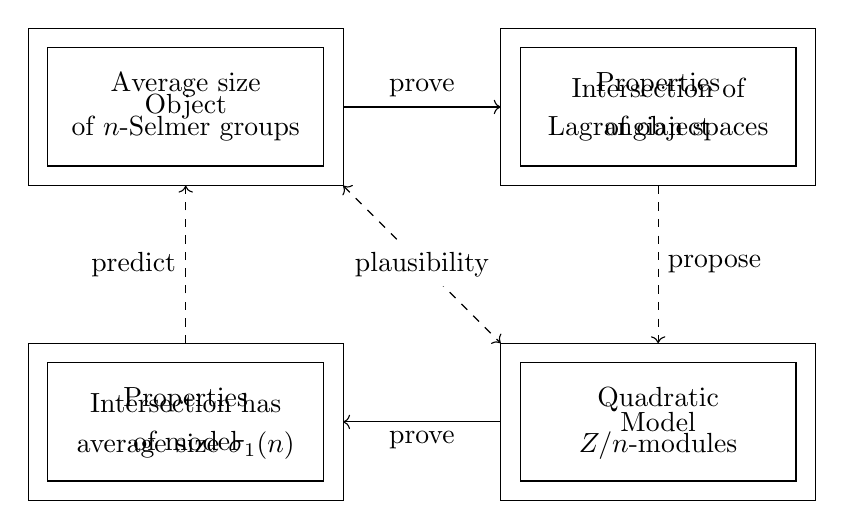
\begin{tikzpicture}
\fill<1> [white] (1, 1) rectangle (5, 3);
\draw<1-6> (-1, 1) rectangle node{Object} (-5, 3);
\draw<2-10> [->] (-1, 2) to node[above]{prove} (1, 2);
\draw<2-7> (1, 1) rectangle node[above]{Properties} node[below]{of object} (5, 3);
\draw<3-10> [->, dashed] (3, 1) to node[right]{propose} (3, -1);
\draw<3-8> (1, -1) rectangle node{Model} (5, -3);
\draw<4-10> [->] (1, -2) to node[below]{prove} (-1, -2);
\draw<4-9> (-1, -1) rectangle node[above]{Properties} node[below]{of model} (-5, -3);
\draw<5-10> [->, dashed] (-3, -1) to node[left]{predict} (-3, 1);
\draw<6-10> [<->, dashed] (-1, 1) to node[fill=white]{plausibility} (1, -1);
\draw<7-10> (-1, 1) rectangle node[above]{Average size} node[below]{of $ n $-Selmer groups} (-5, 3);
\draw<7-10> (-1.25, 1.25) rectangle (-4.75, 2.75);
\draw<8-10> (1, 1) rectangle node[above]{Intersection of} node[below]{Lagrangian spaces} (5, 3);
\draw<8-10> (1.25, 1.25) rectangle (4.75, 2.75);
\draw<9-10> (1, -1) rectangle node[above]{Quadratic} node[below]{$ \mathbb{Z} / n $-modules} (5, -3);
\draw<9-10> (1.25, -1.25) rectangle (4.75, -2.75);
\draw<10> (-1, -1) rectangle node[above]{Intersection has} node[below]{average size $ \sigma_1(n) $} (-5, -3);
\draw<10> (-1.25, -1.25) rectangle (-4.75, -2.75);
\end{tikzpicture}

\end{center}

\only<11-14>{``Modelling the Selmer group, the Tate-Shafarevich group, and the Mordell-Weil rank of elliptic curves over number fields"}

\only<12-14>{
\vspace{0.5cm}
\begin{theorem}[1) (idea]
The $ n $-Selmer group is usually the intersection of two Lagrangian spaces.
\end{theorem}
}

\only<13-14>{
\begin{theorem}[2) (idea]
The intersection of two Lagrangian spaces should have average size $ \sigma_1(n) $.
\end{theorem}
\vspace{0.5cm}
}

\only<14>{``All but finitely many rational elliptic curves have rank at most $ 21 $''}

\end{frame}

\begin{frame}[t]{Preliminary background}

\only<1-7>{Let $ E $ be an \emph{elliptic curve} defined over a \emph{number field} $ K $.}

\only<2-7>{
\begin{itemize}
\item<2-7> $ K $ is a finite extension of $ \mathbb{Q} $ with a fixed algebraic closure $ \overline{K} $.
\item<3-7> $ E = E(\overline{K}) $ is a smooth projective plane curve of genus one with a distinguished point $ \mathcal{O} \in E(K) $.
\item<4-7> $ \operatorname{Gal}(\overline{K} / K) $ acts on $ E $ with invariants $ E(K) $.
\end{itemize}
}

\only<5-7>{
\vspace{0.5cm}
\begin{theorem}[Mordell-Weil]
$ E(K) $ is a finitely generated abelian group.
\end{theorem}
}

\only<6-7>{
\vspace{0.5cm}
There is an isomorphism
$$ E(K) \cong \operatorname{tors}(E / K) \times \mathbb{Z}^{\operatorname{rk}(E / K)}. $$
}%
\only<7>{The \textbf{Mordell-Weil rank} is $ \operatorname{rk}(E / K) $.}

\only<8-22>{Let $ E $ be an elliptic curve defined over a number field $ K $.}

\only<9-11>{
Multiplying by $ n \in \mathbb{N}^+ $,
$$ 0 \to E[n] \to E \xrightarrow{[n]} E \to 0. $$
}%
\only<10-11>{%
Applying $ \operatorname{Gal}(\overline{K} / K) $ cohomology,
$$
\begin{tikzcd}[ampersand replacement=\&, column sep=tiny]
0 \arrow{r} \& E(K)[n] \arrow{r} \& E(K) \arrow{r} \& E(K) \arrow[in=180, out=0]{dll}[swap]{\delta} \& \\
\& H^1(K, E[n]) \arrow{r} \& H^1(K, E) \arrow{r} \& H^1(K, E) \arrow{r} \& \dots.
\end{tikzcd}
$$
}%
\only<11>{%
Truncating at $ H^1(K, E[n]) $,
$$
\begin{tikzcd}[ampersand replacement=\&]
0 \longrightarrow E(K) / n \arrow{r} \& H^1(K, E[n]) \arrow{r} \& H^1(K, E)[n] \longrightarrow 0
\end{tikzcd}.
$$
}

\only<12-16>{
There is a short exact sequence
$$
\begin{tikzcd}[ampersand replacement=\&]
0 \longrightarrow E(K) / n \arrow{r} \& H^1(K, E[n]) \arrow{r} \& H^1(K, E)[n] \longrightarrow 0
\end{tikzcd}.
$$
}

\only<13-16>{Let $ K_v $ be a \emph{completion} of $ K $ with respect to a norm $ |\cdot|_v $.}

\only<14-16>{
\begin{itemize}
\item $ K_v $ is one of $ K_{\mathfrak{p}} $, $ \mathbb{R} $, or $ \mathbb{C} $.
\end{itemize}
}

\only<15>{
Similarly,
$$
\begin{tikzcd}[ampersand replacement=\&, column sep=small]
0 \longrightarrow E(K_v) / n \arrow{r} \& H^1(K_v, E[n]) \arrow{r} \& H^1(K_v, E)[n] \longrightarrow 0
\end{tikzcd}.
$$
}

\only<16>{
Similarly,
$$
\begin{tikzcd}[ampersand replacement=\&, column sep=tiny]
0 \arrow{r} \& \displaystyle\prod_v E(K_v) / n \arrow{r} \& \displaystyle\prod_v H^1(K_v, E[n]) \arrow{r} \& \displaystyle\prod_v H^1(K_v, E)[n] \arrow{r} \& 0
\end{tikzcd}.
$$
}

\only<17>{
There are short exact sequences
$$
\begin{tikzcd}[ampersand replacement=\&]
0 \longrightarrow E(K) / n \arrow{r} \& H^1(K, E[n]) \arrow{r} \& H^1(K, E)[n] \longrightarrow 0
\end{tikzcd},
$$
\vspace{0.05cm}
$$
\begin{tikzcd}[ampersand replacement=\&, column sep=tiny]
0 \arrow{r} \& \displaystyle\prod_v E(K_v) / n \arrow{r} \& \displaystyle\prod_v H^1(K_v, E[n]) \arrow{r} \& \displaystyle\prod_v H^1(K_v, E)[n] \arrow{r} \& 0
\end{tikzcd}.
$$
}

\only<18-22>{
There is a row-exact commutative diagram
$$
\begin{tikzcd}[ampersand replacement=\&, column sep=tiny]
0 \arrow{r} \& E(K) / n \arrow{r} \arrow{d} \& H^1(K, E[n]) \arrow{r} \arrow{d}[swap]{\only<20-22>{\lambda}} \only<19-22>{\arrow[dashed]{dr}{\sigma}} \& H^1(K, E)[n] \arrow{r} \arrow{d}{\only<21-22>{\tau[n]}} \& 0 \\
0 \arrow{r} \& \displaystyle\prod_v E(K_v) / n \arrow{r}[swap]{\only<20-22>\kappa} \& \displaystyle\prod_v H^1(K_v, E[n]) \arrow{r} \& \displaystyle\prod_v H^1(K_v, E)[n] \arrow{r} \& 0
\end{tikzcd}.
$$
}%
\only<19-20>{%
The \textbf{$ n $-Selmer group} is
$$ \mathcal{S}_n(K, E) = \ker (\sigma : H^1(K, E[n]) \to \textstyle\prod_v H^1(K_v, E)[n]). $$
}%
\only<20>{%
By the first isomorphism theorem,
$$ \mathcal{S}_n(K, E) / \ker \lambda \xrightarrow{\sim} \operatorname{im} \kappa \cap \operatorname{im} \lambda. $$
}%
\only<21-22>{%
The \textbf{Tate-Shafarevich group} is
$$ \Sha(K, E) = \ker (\tau : H^1(K, E) \to \textstyle\prod_v H^1(K_v, E)). $$
}%
\only<22>{%
There is an exact sequence
$$ 0 \to E(K) / n \to \mathcal{S}_n(K, E) \to \Sha(K, E)[n] \to 0. $$
}

\end{frame}

\begin{frame}[t]{Arithmetic of Selmer groups}

\begin{theorem}[1]
For almost all elliptic curves defined over a number field, the $ p^e $-Selmer group is the intersection of two Lagrangian direct summands in a non-degenerate quadratic $ \mathbb{Z} / p^e $-module of infinite rank.
\end{theorem}

\only<2-7>{
\begin{itemize}
\item<2-7> \emph{Almost all}: limiting proportion when ordered by height.
\item<3-7> \emph{Quadratic} module $ M $: has a quadratic form $ \omega : M \to \mathbb{Q} / \mathbb{Z} $.
\item<4-7> \emph{Non-degenerate} $ M $: $ M \cong M^\star $.
\item<5-7> \emph{Lagrangian} submodule $ N $: $ \omega(N) = 0 $ and $ N^\perp = N $.
\item<6-7> \emph{Infinite rank}: in terms of generators.
\end{itemize}
}

\only<7>{
Think of $ M = (\mathbb{Z} / p^e)^{2n} $, equipped with hyperbolic quadratic form
$$ (x_1, \dots, x_n, y_1, \dots, y_n) \mapsto \sum_{i = 1}^n x_iy_i, $$
with Lagrangian submodule $ N = (\mathbb{Z} / p^e)^n \oplus 0^n $.
}

\only<8>{
\vspace{0.5cm}
References:
\begin{itemize}
\item Colliot-Th\'el\`ene, Skorobogatov, Swinnerton-Dyer (1998): $ p^e = 2 $ and finite-dimensional construction. \footnote{\tiny J.-L. Colliot-Thelene, A. Skorobogatov and P. Swinnerton-Dyer. 'Hasse principle for pencils of curves of genus one whose Jacobians have rational 2-division points'. In: Invent. Math. 134 (1998)}
\item Bhargava, Kane, Lenstra, Poonen, Rains (2015): general $ p^e $, infinite-rank construction, and generalisations to abelian varieties with arbitrary isogenies over arbitrary global fields. \footnote{\tiny M. Bhargava, D. Kane, H. Lenstra, B. Poonen and E. Rains. 'Modelling the distribution of ranks, Selmer groups, and Shafarevich-Tate groups of elliptic curves'. In: Camb. J. Math. 3 (2015)}
\end{itemize}
}

\only<9-24>{
\begin{proof}[Sketch of proof]
\renewcommand{\qedsymbol}{}
Recall that $ \mathcal{S}_n(K, E) / \ker \lambda \cong \operatorname{im} \kappa \cap \operatorname{im} \lambda $.
\begin{enumerate}
\item<10-24> Construct the local non-degenerate quadratic module.
\only<11-14>{
\begin{itemize}
\item<11-14> Construct $ \Theta $ such that $ 0 \to \overline{K_v}^\times \to \Theta \to E[n] \to 0 $.
\item<12-14> Define $ \operatorname{Ob}_{K_v} : H^1(K_v, E[n]) \to \operatorname{Br} K_v \hookrightarrow \mathbb{Q} / \mathbb{Z} $.
\item<13-14> Prove $ \langle\cdot, \cdot\rangle_{\operatorname{Ob}_{K_v}} = [\cdot, \cdot] \circ \cup $, and deduce $ \operatorname{Ob}_{K_v} $ is a quadratic form.
\item<14> Show non-degeneracy using local duality.
\end{itemize}
}
\item<15-24> Prove $ \operatorname{im} \kappa $ and $ \operatorname{im} \lambda $ are Lagrangian.
\only<16-19>{
\begin{itemize}
\item<16-19> Prove basic properties of Brauer-Severi diagrams to redefine $ \operatorname{Ob}_{K_v} $.
\item<17-19> Define $ M = \overline{\prod_v} H^1(K_v, E[n]) $ and $ \mathfrak{q} = \sum_v \operatorname{inv}_{K_v} \circ \operatorname{Ob}_{K_v} : M \to \mathbb{Q} / \mathbb{Z} $.
\item<18-19> Show $ \operatorname{im} \kappa $ is Lagrangian using B-S diagrams and local duality.
\item<19> Show $ \operatorname{im} \lambda $ is Lagrangian using class field theory and global duality.
\end{itemize}
}
\item<20-24> Prove $ \operatorname{im} \kappa $ and $ \operatorname{im} \lambda $ are direct summands.
\only<21>{
\begin{itemize}
\item<21> Use infinite abelian group theory to characterise direct summands in terms of divisibility-preserving maps and apply global duality.
\end{itemize}
}
\item<22-24> Attain good criterion for $ \ker \lambda = 0 $ when $ n = p^e $.
\only<23-24>{
\begin{itemize}
\item<23-24> Use Chebotarev's density theorem to reduce to $ H_c^1(\operatorname{im} \rho_{E[n]}, E[n]) $ and apply inflation-restriction repeatedly to reduce to $ \operatorname{SL}_2(\mathbb{Z} / n) $.
\item<24> Extract assumption $ \operatorname{SL}_2(\mathbb{Z} / n) \le \operatorname{im} \rho_{E[n]} $ and justify its ubiquity using Hilbert's irreducibility theorem and division polynomials.
$ \square $
\end{itemize}
}
\end{enumerate}
\end{proof}
}

\end{frame}

\begin{frame}[t]{Model for Selmer groups}

\begin{theorem}[2]
The average size of the intersection of two Lagrangian direct summands of the quadratic $ \mathbb{Z} / p^e $-module $ (\mathbb{Z} / p^e)^{2n} $ chosen uniformly at random tends to the sum of divisors $ \sigma_1 $ of $ p^e $ as $ n \to \infty $.
\end{theorem}

\only<2-5>{
\begin{itemize}
\item<2-5> Theorem (1): the $ p^e $-Selmer group is the intersections of two Lagrangian direct summands in $ \overline{\prod_v} H^1(K_v, E[p^e]) $.
\item<3-5> Theorem (2): the size of the intersection of two Lagrangian direct summands in $ (\mathbb{Z} / p^e)^\infty $ has first moment $ \sigma_1(p^e) $.
\item<4-5> On the other hand, $ (\mathbb{Z} / p^e)^\infty $ is always free, while $ \overline{\prod_v} H^1(K_v, E[p^e]) $ is almost never free, by Hilbert's irreducibility theorem.
\end{itemize}
}

\only<5>{
\vspace{0.5cm}
Reference:
\begin{itemize}
\item Poonen, Rains (2012): $ e = 1 $. \footnote{\tiny B. Poonen and E. Rains. 'Random maximal isotropic subspaces and Selmer groups'. In: J. Amer. Math. Soc 25 (2012)}
\end{itemize}
}

\only<6-18>{
\begin{proof}[Sketch of proof]
\renewcommand{\qedsymbol}{}
Crucial assumption of direct summands.
\begin{enumerate}
\item<7-18> Linear algebra of $ (\mathbb{Z} / p^e)^{2n} $.
\only<8-10>{
\begin{itemize}
\item<8-10> Show correspondence theorem for direct summands.
\item<9-10> Count number of direct summands of fixed rank.
\item<10> Obtain linear algebra for Lagrangian direct summands.
\end{itemize}
}
\item<11-18> Lagrangian direct summands of $ (\mathbb{Z} / p^e)^{2n} $.
\only<12-14>{
\begin{itemize}
\item<12-14> Compute result for $ n = 1 $ explicitly.
\item<13-14> Count fibres of $ L \mapsto (L \cap N^\perp + N) / N $.
\item<14> Extract rank one free submodule and apply induction.
\end{itemize}
}
\item<15-18> Average size of $ L_1 \cap L_2 $.
\only<16-18>{
\begin{itemize}
\item<16-18> Count number of injections $ \mathbb{Z} / p^e \hookrightarrow L_1 $.
\item<17-18> Compute probability that $ L_2 $ contains image of $ \mathbb{Z} / p^e \hookrightarrow L_1 $.
\item<18> Deduce result by telescoping argument.
$ \square $
\end{itemize}
}
\end{enumerate}
\end{proof}
}

\end{frame}

\begin{frame}[t]{Heuristic consequences}

A model for $ n $-Selmer groups.

\only<2-6>{
\begin{itemize}
\item<2-6> For almost all elliptic curves $ E $ defined over a number field $ K $,
$$ \mathcal{S}_n(K, E)[p^e] \cong \mathcal{S}_{p^e}(K, E), \qquad p^e \mid n. $$
\item<3-6> Derive linear algebra for $ \mathbb{Z} / n $ and consider $ (L_1 \cap L_2)[p^e] $.
\end{itemize}
}

\only<4-6>{
\vspace{0.5cm}
A model for Mordell-Weil ranks and Tate-Shafarevich groups.
}

\only<5-6>{
\begin{itemize}
\item<5-6> Use
$$ 0 \to E(K) \otimes \mathbb{Q}_p / \mathbb{Z}_p \to \varinjlim_e \mathcal{S}_{p^e}(K, E) \to \Sha(K, E)[p^\infty] \to 0. $$
\item<6> Consider
$$ 0 \to (L_1 \cap L_2) \otimes \mathbb{Q}_p / \mathbb{Z}_p \to (L_1 \otimes \mathbb{Q}_p / \mathbb{Z}_p) \cap (L_2 \otimes \mathbb{Q}_p / \mathbb{Z}_p) \to T \to 0. $$
\end{itemize}
}

\end{frame}

\begin{frame}

\begin{center}

{\Huge THANK YOU}

\end{center}

\end{frame}

\end{document}